\documentclass{article}
\usepackage[T1]{fontenc}
\usepackage{lmodern}
\usepackage{graphicx}
\usepackage{amsmath,amssymb}
\usepackage[a4paper,margin=2cm]{geometry}
\usepackage[absolute,overlay]{textpos}
\setlength{\TPHorizModule}{1mm}
\setlength{\TPVertModule}{1mm}
\usepackage[indonesian]{babel}
\usepackage{hyperref}
\setlength{\emergencystretch}{2em}
% unit: Halaman 42

\begin{document}

% === Halaman 42 (llm) ===

\vspace{146.72mm}

\section*{Acoustic Eavesdropping}

\vspace{10mm}

% deskripsi: Ilustrasi seseorang yang bersembunyi di bawah meja untuk mendengarkan percakapan menggunakan alat perekam dan mikrofon.
% bbox normalisasi: [0.1480, 0.2470, 0.4080, 0.8330]
\begin{textblock*}{54.60mm}(31.08mm,73.36mm)
\noindent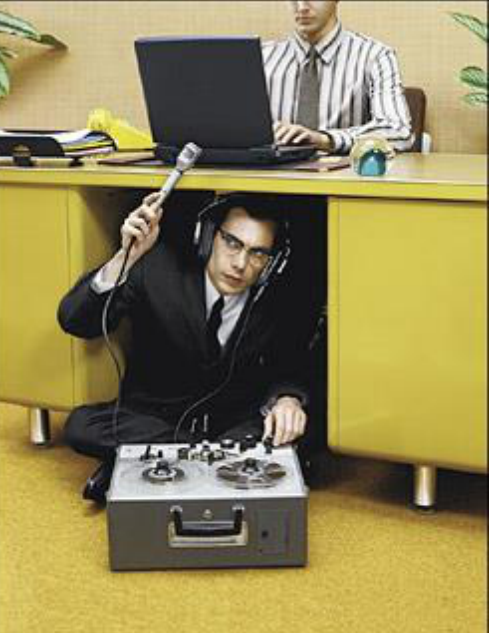
\includegraphics[width=54.60mm,height=174.04mm]{../../images/llm/page_042_img_01.png}%
\end{textblock*}

% deskripsi: Ilustrasi seseorang yang bersembunyi di bawah meja kantor sementara orang lain sedang berbicara di telepon di atas meja.
% bbox normalisasi: [0.4650, 0.2470, 0.8840, 0.7410]
\begin{textblock*}{87.99mm}(97.65mm,73.36mm)
\noindent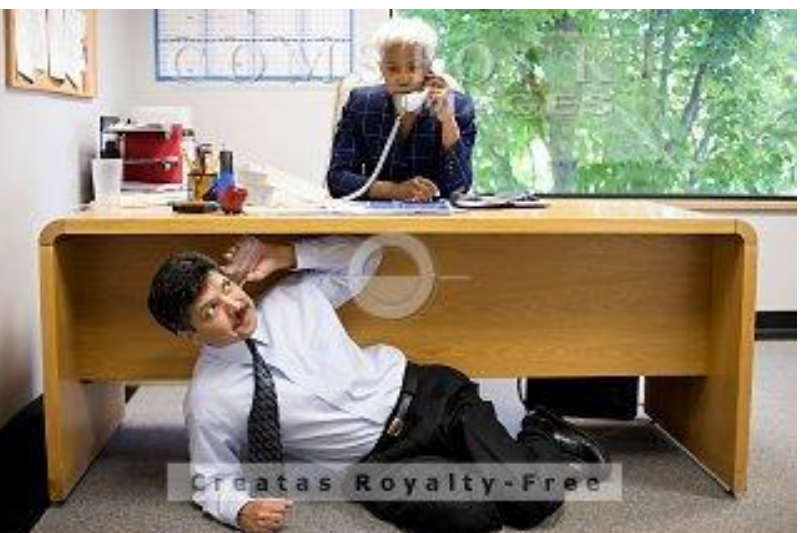
\includegraphics[width=87.99mm,height=146.72mm]{../../images/llm/page_042_img_02.png}%
\end{textblock*}

\end{document}
